\documentclass[1p]{elsarticle_modified}
%\bibliographystyle{elsarticle-num}

%\usepackage[colorlinks]{hyperref}
%\usepackage{abbrmath_seonhwa} %\Abb, \Ascr, \Acal ,\Abf, \Afrak
\usepackage{amsfonts}
\usepackage{amssymb}
\usepackage{amsmath}
\usepackage{amsthm}
\usepackage{scalefnt}
\usepackage{amsbsy}
\usepackage{kotex}
\usepackage{caption}
\usepackage{subfig}
\usepackage{color}
\usepackage{graphicx}
\usepackage{xcolor} %% white, black, red, green, blue, cyan, magenta, yellow
\usepackage{float}
\usepackage{setspace}
\usepackage{hyperref}

\usepackage{tikz}
\usetikzlibrary{arrows}

\usepackage{multirow}
\usepackage{array} % fixed length table
\usepackage{hhline}

%%%%%%%%%%%%%%%%%%%%%
\makeatletter
\renewcommand*\env@matrix[1][\arraystretch]{%
	\edef\arraystretch{#1}%
	\hskip -\arraycolsep
	\let\@ifnextchar\new@ifnextchar
	\array{*\c@MaxMatrixCols c}}
\makeatother %https://tex.stackexchange.com/questions/14071/how-can-i-increase-the-line-spacing-in-a-matrix
%%%%%%%%%%%%%%%

\usepackage[normalem]{ulem}

\newcommand{\msout}[1]{\ifmmode\text{\sout{\ensuremath{#1}}}\else\sout{#1}\fi}
%SOURCE: \msout is \stkout macro in https://tex.stackexchange.com/questions/20609/strikeout-in-math-mode

\newcommand{\cancel}[1]{
	\ifmmode
	{\color{red}\msout{#1}}
	\else
	{\color{red}\sout{#1}}
	\fi
}

\newcommand{\add}[1]{
	{\color{blue}\uwave{#1}}
}

\newcommand{\replace}[2]{
	\ifmmode
	{\color{red}\msout{#1}}{\color{blue}\uwave{#2}}
	\else
	{\color{red}\sout{#1}}{\color{blue}\uwave{#2}}
	\fi
}

\newcommand{\Sol}{\mathcal{S}} %segment
\newcommand{\D}{D} %diagram
\newcommand{\A}{\mathcal{A}} %arc


%%%%%%%%%%%%%%%%%%%%%%%%%%%%%5 test

\def\sl{\operatorname{\textup{SL}}(2,\Cbb)}
\def\psl{\operatorname{\textup{PSL}}(2,\Cbb)}
\def\quan{\mkern 1mu \triangleright \mkern 1mu}

\theoremstyle{definition}
\newtheorem{thm}{Theorem}[section]
\newtheorem{prop}[thm]{Proposition}
\newtheorem{lem}[thm]{Lemma}
\newtheorem{ques}[thm]{Question}
\newtheorem{cor}[thm]{Corollary}
\newtheorem{defn}[thm]{Definition}
\newtheorem{exam}[thm]{Example}
\newtheorem{rmk}[thm]{Remark}
\newtheorem{alg}[thm]{Algorithm}

\newcommand{\I}{\sqrt{-1}}
\begin{document}

%\begin{frontmatter}
%
%\title{Boundary parabolic representations of knots up to 8 crossings}
%
%%% Group authors per affiliation:
%\author{Yunhi Cho} 
%\address{Department of Mathematics, University of Seoul, Seoul, Korea}
%\ead{yhcho@uos.ac.kr}
%
%
%\author{Seonhwa Kim} %\fnref{s_kim}}
%\address{Center for Geometry and Physics, Institute for Basic Science, Pohang, 37673, Korea}
%\ead{ryeona17@ibs.re.kr}
%
%\author{Hyuk Kim}
%\address{Department of Mathematical Sciences, Seoul National University, Seoul 08826, Korea}
%\ead{hyukkim@snu.ac.kr}
%
%\author{Seokbeom Yoon}
%\address{Department of Mathematical Sciences, Seoul National University, Seoul, 08826,  Korea}
%\ead{sbyoon15@snu.ac.kr}
%
%\begin{abstract}
%We find all boundary parabolic representation of knots up to 8 crossings.
%
%\end{abstract}
%\begin{keyword}
%    \MSC[2010] 57M25 
%\end{keyword}
%
%\end{frontmatter}

%\linenumbers
%\tableofcontents
%
\newcommand\colored[1]{\textcolor{white}{\rule[-0.35ex]{0.8em}{1.4ex}}\kern-0.8em\color{red} #1}%
%\newcommand\colored[1]{\textcolor{white}{ #1}\kern-2.17ex	\textcolor{white}{ #1}\kern-1.81ex	\textcolor{white}{ #1}\kern-2.15ex\color{red}#1	}

{\Large $\underline{11a_{27}~(K11a_{27})}$}

\setlength{\tabcolsep}{10pt}
\renewcommand{\arraystretch}{1.6}
\vspace{1cm}\begin{tabular}{m{100pt}>{\centering\arraybackslash}m{274pt}}
\multirow{5}{120pt}{
	\centering
	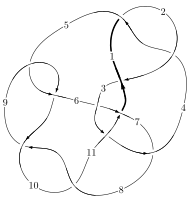
\includegraphics[width=112pt]{../../../GIT/diagram.site/Diagrams/png/276_11a_27.png}\\
\ \ \ A knot diagram\footnotemark}&
\allowdisplaybreaks
\textbf{Linearized knot diagam} \\
\cline{2-2}
 &
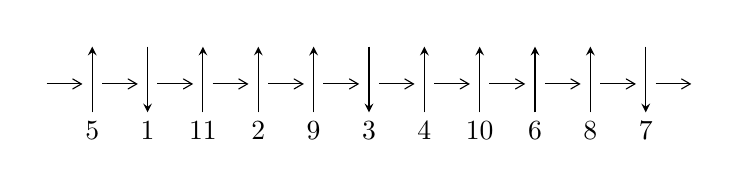
\begin{tikzpicture}[x=20pt, y=17pt]
	% nodes
	\node (C0) at (0, 0) {};
	\node (C1) at (1, 0) {};
	\node (C1U) at (1, +1) {};
	\node (C1D) at (1, -1) {5};

	\node (C2) at (2, 0) {};
	\node (C2U) at (2, +1) {};
	\node (C2D) at (2, -1) {1};

	\node (C3) at (3, 0) {};
	\node (C3U) at (3, +1) {};
	\node (C3D) at (3, -1) {11};

	\node (C4) at (4, 0) {};
	\node (C4U) at (4, +1) {};
	\node (C4D) at (4, -1) {2};

	\node (C5) at (5, 0) {};
	\node (C5U) at (5, +1) {};
	\node (C5D) at (5, -1) {9};

	\node (C6) at (6, 0) {};
	\node (C6U) at (6, +1) {};
	\node (C6D) at (6, -1) {3};

	\node (C7) at (7, 0) {};
	\node (C7U) at (7, +1) {};
	\node (C7D) at (7, -1) {4};

	\node (C8) at (8, 0) {};
	\node (C8U) at (8, +1) {};
	\node (C8D) at (8, -1) {10};

	\node (C9) at (9, 0) {};
	\node (C9U) at (9, +1) {};
	\node (C9D) at (9, -1) {6};

	\node (C10) at (10, 0) {};
	\node (C10U) at (10, +1) {};
	\node (C10D) at (10, -1) {8};

	\node (C11) at (11, 0) {};
	\node (C11U) at (11, +1) {};
	\node (C11D) at (11, -1) {7};
	\node (C12) at (12, 0) {};

	% arrows
	\draw[->,>={angle 60}]
	(C0) edge (C1) (C1) edge (C2) (C2) edge (C3) (C3) edge (C4) (C4) edge (C5) (C5) edge (C6) (C6) edge (C7) (C7) edge (C8) (C8) edge (C9) (C9) edge (C10) (C10) edge (C11) (C11) edge (C12) ;	\draw[->,>=stealth]
	(C1D) edge (C1U) (C2U) edge (C2D) (C3D) edge (C3U) (C4D) edge (C4U) (C5D) edge (C5U) (C6U) edge (C6D) (C7D) edge (C7U) (C8D) edge (C8U) (C9D) edge (C9U) (C10D) edge (C10U) (C11U) edge (C11D) ;
	\end{tikzpicture} \\
\hhline{~~} \\& 
\textbf{Solving Sequence} \\ \cline{2-2} 
 &
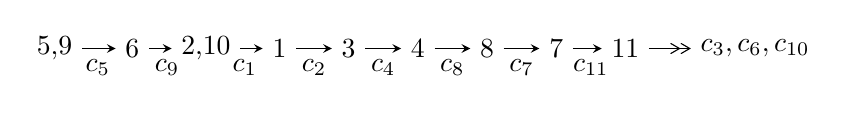
\begin{tikzpicture}[x=25pt, y=7pt]
	% node
	\node (A0) at (-1/8, 0) {5,9};
	\node (A1) at (1, 0) {6};
	\node (A2) at (33/16, 0) {2,10};
	\node (A3) at (25/8, 0) {1};
	\node (A4) at (33/8, 0) {3};
	\node (A5) at (41/8, 0) {4};
	\node (A6) at (49/8, 0) {8};
	\node (A7) at (57/8, 0) {7};
	\node (A8) at (65/8, 0) {11};
	\node (C1) at (1/2, -1) {$c_{5}$};
	\node (C2) at (3/2, -1) {$c_{9}$};
	\node (C3) at (21/8, -1) {$c_{1}$};
	\node (C4) at (29/8, -1) {$c_{2}$};
	\node (C5) at (37/8, -1) {$c_{4}$};
	\node (C6) at (45/8, -1) {$c_{8}$};
	\node (C7) at (53/8, -1) {$c_{7}$};
	\node (C8) at (61/8, -1) {$c_{11}$};
	\node (A9) at (10, 0) {$c_{3},c_{6},c_{10}$};

	% edge
	\draw[->,>=stealth]	
	(A0) edge (A1) (A1) edge (A2) (A2) edge (A3) (A3) edge (A4) (A4) edge (A5) (A5) edge (A6) (A6) edge (A7) (A7) edge (A8) ;
	\draw[->>,>={angle 60}]	
	(A8) edge (A9);
\end{tikzpicture} \\ 

\end{tabular} \\

\footnotetext{
The image of knot diagram is generated by the software ``\textbf{Draw programme}" developed by Andrew Bartholomew(\url{http://www.layer8.co.uk/maths/draw/index.htm\#Running-draw}), where we modified some parts for our purpose(\url{https://github.com/CATsTAILs/LinksPainter}).
}\phantom \\ \newline 
\centering \textbf{Ideals for irreducible components\footnotemark of $X_{\text{par}}$} 
 
\begin{align*}
I^u_{1}&=\langle 
-5.81141\times10^{45} u^{72}-2.55560\times10^{45} u^{71}+\cdots+5.58876\times10^{45} b+1.50088\times10^{46},\\
\phantom{I^u_{1}}&\phantom{= \langle  }1.50317\times10^{47} u^{72}+3.46308\times10^{47} u^{71}+\cdots+5.58876\times10^{45} a+2.41035\times10^{47},\;u^{73}+3 u^{72}+\cdots+8 u+1\rangle \\
I^u_{2}&=\langle 
b+a+1,\;a^2+3 a+3,\;u+1\rangle \\
\\
\end{align*}
\raggedright * 2 irreducible components of $\dim_{\mathbb{C}}=0$, with total 75 representations.\\
\footnotetext{All coefficients of polynomials are rational numbers. But the coefficients are sometimes approximated in decimal forms when there is not enough margin.}
\newpage
\renewcommand{\arraystretch}{1}
\centering \section*{I. $I^u_{1}= \langle -5.81\times10^{45} u^{72}-2.56\times10^{45} u^{71}+\cdots+5.59\times10^{45} b+1.50\times10^{46},\;1.50\times10^{47} u^{72}+3.46\times10^{47} u^{71}+\cdots+5.59\times10^{45} a+2.41\times10^{47},\;u^{73}+3 u^{72}+\cdots+8 u+1 \rangle$}
\flushleft \textbf{(i) Arc colorings}\\
\begin{tabular}{m{7pt} m{180pt} m{7pt} m{180pt} }
\flushright $a_{5}=$&$\begin{pmatrix}1\\0\end{pmatrix}$ \\
\flushright $a_{9}=$&$\begin{pmatrix}0\\u\end{pmatrix}$ \\
\flushright $a_{6}=$&$\begin{pmatrix}1\\- u^2\end{pmatrix}$ \\
\flushright $a_{2}=$&$\begin{pmatrix}-26.8963 u^{72}-61.9652 u^{71}+\cdots-262.686 u-43.1285\\1.03984 u^{72}+0.457276 u^{71}+\cdots-8.76067 u-2.68554\end{pmatrix}$ \\
\flushright $a_{10}=$&$\begin{pmatrix}u\\- u^3+u\end{pmatrix}$ \\
\flushright $a_{1}=$&$\begin{pmatrix}-27.9361 u^{72}-62.4224 u^{71}+\cdots-253.925 u-40.4429\\1.03984 u^{72}+0.457276 u^{71}+\cdots-8.76067 u-2.68554\end{pmatrix}$ \\
\flushright $a_{3}=$&$\begin{pmatrix}-55.1885 u^{72}-128.039 u^{71}+\cdots-541.292 u-84.5791\\-0.557631 u^{72}-3.16857 u^{71}+\cdots-25.1345 u-4.27345\end{pmatrix}$ \\
\flushright $a_{4}=$&$\begin{pmatrix}52.9421 u^{72}+122.525 u^{71}+\cdots+513.869 u+80.0761\\-0.291491 u^{72}+0.944537 u^{71}+\cdots+12.7180 u+2.20055\end{pmatrix}$ \\
\flushright $a_{8}=$&$\begin{pmatrix}- u^3\\u^5- u^3+u\end{pmatrix}$ \\
\flushright $a_{7}=$&$\begin{pmatrix}54.1305 u^{72}+120.249 u^{71}+\cdots+492.164 u+73.9005\\-11.1367 u^{72}-24.4194 u^{71}+\cdots-88.7848 u-13.4461\end{pmatrix}$ \\
\flushright $a_{11}=$&$\begin{pmatrix}u^5+u\\- u^7+u^5-2 u^3+u\end{pmatrix}$\\ \flushright $a_{11}=$&$\begin{pmatrix}u^5+u\\- u^7+u^5-2 u^3+u\end{pmatrix}$\\&\end{tabular}
\flushleft \textbf{(ii) Obstruction class $= -1$}\\~\\
\flushleft \textbf{(iii) Cusp Shapes $= -73.5210 u^{72}-182.862 u^{71}+\cdots-811.040 u-125.700$}\\~\\
\newpage\renewcommand{\arraystretch}{1}
\flushleft \textbf{(iv) u-Polynomials at the component}\newline \\
\begin{tabular}{m{50pt}|m{274pt}}
Crossings & \hspace{64pt}u-Polynomials at each crossing \\
\hline $$\begin{aligned}c_{1},c_{4}\end{aligned}$$&$\begin{aligned}
&u^{73}+2 u^{72}+\cdots+7 u-1
\end{aligned}$\\
\hline $$\begin{aligned}c_{2}\end{aligned}$$&$\begin{aligned}
&u^{73}+32 u^{72}+\cdots+131 u-1
\end{aligned}$\\
\hline $$\begin{aligned}c_{3}\end{aligned}$$&$\begin{aligned}
&u^{73}+7 u^{72}+\cdots+12 u+4
\end{aligned}$\\
\hline $$\begin{aligned}c_{5},c_{9}\end{aligned}$$&$\begin{aligned}
&u^{73}-3 u^{72}+\cdots+8 u-1
\end{aligned}$\\
\hline $$\begin{aligned}c_{6}\end{aligned}$$&$\begin{aligned}
&u^{73}+34 u^{71}+\cdots-149 u-41
\end{aligned}$\\
\hline $$\begin{aligned}c_{7}\end{aligned}$$&$\begin{aligned}
&u^{73}-2 u^{72}+\cdots-784 u-224
\end{aligned}$\\
\hline $$\begin{aligned}c_{8},c_{10}\end{aligned}$$&$\begin{aligned}
&u^{73}-23 u^{72}+\cdots-2 u-1
\end{aligned}$\\
\hline $$\begin{aligned}c_{11}\end{aligned}$$&$\begin{aligned}
&u^{73}-7 u^{72}+\cdots- u^2-1
\end{aligned}$\\
\hline
\end{tabular}\\~\\
\newpage\renewcommand{\arraystretch}{1}
\flushleft \textbf{(v) Riley Polynomials at the component}\newline \\
\begin{tabular}{m{50pt}|m{274pt}}
Crossings & \hspace{64pt}Riley Polynomials at each crossing \\
\hline $$\begin{aligned}c_{1},c_{4}\end{aligned}$$&$\begin{aligned}
&y^{73}+32 y^{72}+\cdots+131 y-1
\end{aligned}$\\
\hline $$\begin{aligned}c_{2}\end{aligned}$$&$\begin{aligned}
&y^{73}+20 y^{72}+\cdots+19907 y-1
\end{aligned}$\\
\hline $$\begin{aligned}c_{3}\end{aligned}$$&$\begin{aligned}
&y^{73}+15 y^{72}+\cdots-344 y-16
\end{aligned}$\\
\hline $$\begin{aligned}c_{5},c_{9}\end{aligned}$$&$\begin{aligned}
&y^{73}-23 y^{72}+\cdots-2 y-1
\end{aligned}$\\
\hline $$\begin{aligned}c_{6}\end{aligned}$$&$\begin{aligned}
&y^{73}+68 y^{72}+\cdots-11173 y-1681
\end{aligned}$\\
\hline $$\begin{aligned}c_{7}\end{aligned}$$&$\begin{aligned}
&y^{73}+84 y^{72}+\cdots-1858304 y-50176
\end{aligned}$\\
\hline $$\begin{aligned}c_{8},c_{10}\end{aligned}$$&$\begin{aligned}
&y^{73}+57 y^{72}+\cdots+254 y-1
\end{aligned}$\\
\hline $$\begin{aligned}c_{11}\end{aligned}$$&$\begin{aligned}
&y^{73}+5 y^{72}+\cdots-2 y-1
\end{aligned}$\\
\hline
\end{tabular}\\~\\
\newpage\flushleft \textbf{(vi) Complex Volumes and Cusp Shapes}
$$\begin{array}{c|c|c}  
\text{Solutions to }I^u_{1}& \I (\text{vol} + \sqrt{-1}CS) & \text{Cusp shape}\\
 \hline 
\begin{aligned}
u &= \phantom{-}0.872133 + 0.330890 I \\
a &= \phantom{-}0.347576 - 0.582681 I \\
b &= -0.093427 - 1.105170 I\end{aligned}
 & -1.56864 + 4.14463 I & \phantom{-0.000000 } 0. - 8.01358 I \\ \hline\begin{aligned}
u &= \phantom{-}0.872133 - 0.330890 I \\
a &= \phantom{-}0.347576 + 0.582681 I \\
b &= -0.093427 + 1.105170 I\end{aligned}
 & -1.56864 - 4.14463 I & \phantom{-0.000000 -}0. + 8.01358 I \\ \hline\begin{aligned}
u &= -0.827433 + 0.687248 I \\
a &= -0.757692 - 0.116396 I \\
b &= -0.903670 - 0.847810 I\end{aligned}
 & -0.261500 + 0.649592 I & \phantom{-0.000000 } 0 \\ \hline\begin{aligned}
u &= -0.827433 - 0.687248 I \\
a &= -0.757692 + 0.116396 I \\
b &= -0.903670 + 0.847810 I\end{aligned}
 & -0.261500 - 0.649592 I & \phantom{-0.000000 } 0 \\ \hline\begin{aligned}
u &= \phantom{-}0.917251 + 0.028799 I \\
a &= \phantom{-}0.957675 + 0.465286 I \\
b &= -0.899692 - 0.482863 I\end{aligned}
 & \phantom{-}4.06916 + 1.66774 I & \phantom{-}17.5628 - 3.8525 I \\ \hline\begin{aligned}
u &= \phantom{-}0.917251 - 0.028799 I \\
a &= \phantom{-}0.957675 - 0.465286 I \\
b &= -0.899692 + 0.482863 I\end{aligned}
 & \phantom{-}4.06916 - 1.66774 I & \phantom{-}17.5628 + 3.8525 I \\ \hline\begin{aligned}
u &= \phantom{-}0.744709 + 0.796357 I \\
a &= -0.254774 + 0.121438 I \\
b &= \phantom{-}0.525153 + 0.176233 I\end{aligned}
 & -3.74839 + 1.23253 I & \phantom{-0.000000 } 0 \\ \hline\begin{aligned}
u &= \phantom{-}0.744709 - 0.796357 I \\
a &= -0.254774 - 0.121438 I \\
b &= \phantom{-}0.525153 - 0.176233 I\end{aligned}
 & -3.74839 - 1.23253 I & \phantom{-0.000000 } 0 \\ \hline\begin{aligned}
u &= -0.797947 + 0.753369 I \\
a &= -0.64416 - 1.83433 I \\
b &= -0.572115 - 1.246620 I\end{aligned}
 & -3.09906 + 2.70236 I & \phantom{-0.000000 } 0 \\ \hline\begin{aligned}
u &= -0.797947 - 0.753369 I \\
a &= -0.64416 + 1.83433 I \\
b &= -0.572115 + 1.246620 I\end{aligned}
 & -3.09906 - 2.70236 I & \phantom{-0.000000 } 0\\
 \hline 
 \end{array}$$\newpage$$\begin{array}{c|c|c}  
\text{Solutions to }I^u_{1}& \I (\text{vol} + \sqrt{-1}CS) & \text{Cusp shape}\\
 \hline 
\begin{aligned}
u &= \phantom{-}1.077830 + 0.219114 I \\
a &= -0.690643 + 0.625004 I \\
b &= \phantom{-}0.817817 - 0.515578 I\end{aligned}
 & \phantom{-}4.44539 + 5.47964 I & \phantom{-0.000000 } 0 \\ \hline\begin{aligned}
u &= \phantom{-}1.077830 - 0.219114 I \\
a &= -0.690643 - 0.625004 I \\
b &= \phantom{-}0.817817 + 0.515578 I\end{aligned}
 & \phantom{-}4.44539 - 5.47964 I & \phantom{-0.000000 } 0 \\ \hline\begin{aligned}
u &= \phantom{-}0.887299 + 0.116247 I \\
a &= \phantom{-}1.69631 - 0.07268 I \\
b &= -0.704741 - 1.080540 I\end{aligned}
 & \phantom{-}2.29836 + 4.22810 I & \phantom{-}12.1430 - 9.3439 I \\ \hline\begin{aligned}
u &= \phantom{-}0.887299 - 0.116247 I \\
a &= \phantom{-}1.69631 + 0.07268 I \\
b &= -0.704741 + 1.080540 I\end{aligned}
 & \phantom{-}2.29836 - 4.22810 I & \phantom{-}12.1430 + 9.3439 I \\ \hline\begin{aligned}
u &= -0.880598 + 0.669028 I \\
a &= -0.700925 + 0.813755 I \\
b &= -0.964342 - 0.090780 I\end{aligned}
 & \phantom{-}0.69933 - 2.58301 I & \phantom{-0.000000 } 0 \\ \hline\begin{aligned}
u &= -0.880598 - 0.669028 I \\
a &= -0.700925 - 0.813755 I \\
b &= -0.964342 + 0.090780 I\end{aligned}
 & \phantom{-}0.69933 + 2.58301 I & \phantom{-0.000000 } 0 \\ \hline\begin{aligned}
u &= \phantom{-}0.875902 + 0.690173 I \\
a &= -0.191233 + 0.289860 I \\
b &= -0.386326 - 0.616731 I\end{aligned}
 & -2.40217 + 4.04097 I & \phantom{-0.000000 } 0 \\ \hline\begin{aligned}
u &= \phantom{-}0.875902 - 0.690173 I \\
a &= -0.191233 - 0.289860 I \\
b &= -0.386326 + 0.616731 I\end{aligned}
 & -2.40217 - 4.04097 I & \phantom{-0.000000 } 0 \\ \hline\begin{aligned}
u &= \phantom{-}0.668112 + 0.895781 I \\
a &= -0.28502 - 1.45618 I \\
b &= \phantom{-}0.465696 - 1.063540 I\end{aligned}
 & -6.08025 - 2.66865 I & \phantom{-0.000000 } 0 \\ \hline\begin{aligned}
u &= \phantom{-}0.668112 - 0.895781 I \\
a &= -0.28502 + 1.45618 I \\
b &= \phantom{-}0.465696 + 1.063540 I\end{aligned}
 & -6.08025 + 2.66865 I & \phantom{-0.000000 } 0\\
 \hline 
 \end{array}$$\newpage$$\begin{array}{c|c|c}  
\text{Solutions to }I^u_{1}& \I (\text{vol} + \sqrt{-1}CS) & \text{Cusp shape}\\
 \hline 
\begin{aligned}
u &= -0.720415 + 0.855626 I \\
a &= \phantom{-}0.314675 - 0.528100 I \\
b &= \phantom{-}0.910054 - 0.387571 I\end{aligned}
 & -2.75982 + 5.17856 I & \phantom{-0.000000 } 0 \\ \hline\begin{aligned}
u &= -0.720415 - 0.855626 I \\
a &= \phantom{-}0.314675 + 0.528100 I \\
b &= \phantom{-}0.910054 + 0.387571 I\end{aligned}
 & -2.75982 - 5.17856 I & \phantom{-0.000000 } 0 \\ \hline\begin{aligned}
u &= \phantom{-}0.876241 + 0.702164 I \\
a &= -0.81649 - 1.39051 I \\
b &= -0.484219 + 0.695912 I\end{aligned}
 & -2.39394 + 1.31325 I & \phantom{-0.000000 } 0 \\ \hline\begin{aligned}
u &= \phantom{-}0.876241 - 0.702164 I \\
a &= -0.81649 + 1.39051 I \\
b &= -0.484219 - 0.695912 I\end{aligned}
 & -2.39394 - 1.31325 I & \phantom{-0.000000 } 0 \\ \hline\begin{aligned}
u &= \phantom{-}0.846597 + 0.756952 I \\
a &= \phantom{-}0.55091 + 3.03768 I \\
b &= -0.468658 + 0.954426 I\end{aligned}
 & -3.36772 + 0.28806 I & \phantom{-0.000000 } 0 \\ \hline\begin{aligned}
u &= \phantom{-}0.846597 - 0.756952 I \\
a &= \phantom{-}0.55091 - 3.03768 I \\
b &= -0.468658 - 0.954426 I\end{aligned}
 & -3.36772 - 0.28806 I & \phantom{-0.000000 } 0 \\ \hline\begin{aligned}
u &= -1.070550 + 0.396975 I \\
a &= -1.34075 - 0.70080 I \\
b &= \phantom{-}0.606073 - 0.641390 I\end{aligned}
 & \phantom{-}3.44487 - 1.41386 I & \phantom{-0.000000 } 0 \\ \hline\begin{aligned}
u &= -1.070550 - 0.396975 I \\
a &= -1.34075 + 0.70080 I \\
b &= \phantom{-}0.606073 + 0.641390 I\end{aligned}
 & \phantom{-}3.44487 + 1.41386 I & \phantom{-0.000000 } 0 \\ \hline\begin{aligned}
u &= -0.853435\phantom{ +0.000000I} \\
a &= -0.672147\phantom{ +0.000000I} \\
b &= -0.0841487\phantom{ +0.000000I}\end{aligned}
 & \phantom{-}1.41721\phantom{ +0.000000I} & \phantom{-}6.25420\phantom{ +0.000000I} \\ \hline\begin{aligned}
u &= -0.914329 + 0.693377 I \\
a &= \phantom{-}0.55780 + 1.40502 I \\
b &= -0.961681 + 0.764182 I\end{aligned}
 & \phantom{-}0.01661 - 5.97370 I & \phantom{-0.000000 } 0\\
 \hline 
 \end{array}$$\newpage$$\begin{array}{c|c|c}  
\text{Solutions to }I^u_{1}& \I (\text{vol} + \sqrt{-1}CS) & \text{Cusp shape}\\
 \hline 
\begin{aligned}
u &= -0.914329 - 0.693377 I \\
a &= \phantom{-}0.55780 - 1.40502 I \\
b &= -0.961681 - 0.764182 I\end{aligned}
 & \phantom{-}0.01661 + 5.97370 I & \phantom{-0.000000 } 0 \\ \hline\begin{aligned}
u &= -0.720406 + 0.896299 I \\
a &= -0.02381 + 1.65621 I \\
b &= \phantom{-}0.636841 + 1.154700 I\end{aligned}
 & -5.08354 + 10.84060 I & \phantom{-0.000000 } 0 \\ \hline\begin{aligned}
u &= -0.720406 - 0.896299 I \\
a &= -0.02381 - 1.65621 I \\
b &= \phantom{-}0.636841 - 1.154700 I\end{aligned}
 & -5.08354 - 10.84060 I & \phantom{-0.000000 } 0 \\ \hline\begin{aligned}
u &= \phantom{-}1.123670 + 0.265577 I \\
a &= -1.65424 + 0.52442 I \\
b &= \phantom{-}0.645150 + 1.076090 I\end{aligned}
 & \phantom{-}2.75520 + 10.95230 I & \phantom{-0.000000 } 0 \\ \hline\begin{aligned}
u &= \phantom{-}1.123670 - 0.265577 I \\
a &= -1.65424 - 0.52442 I \\
b &= \phantom{-}0.645150 - 1.076090 I\end{aligned}
 & \phantom{-}2.75520 - 10.95230 I & \phantom{-0.000000 } 0 \\ \hline\begin{aligned}
u &= -0.797794 + 0.839281 I \\
a &= -0.62268 - 2.20338 I \\
b &= \phantom{-}0.105796 - 1.302560 I\end{aligned}
 & -8.72144 + 2.03741 I & \phantom{-0.000000 } 0 \\ \hline\begin{aligned}
u &= -0.797794 - 0.839281 I \\
a &= -0.62268 + 2.20338 I \\
b &= \phantom{-}0.105796 + 1.302560 I\end{aligned}
 & -8.72144 - 2.03741 I & \phantom{-0.000000 } 0 \\ \hline\begin{aligned}
u &= -0.056905 + 0.832963 I \\
a &= -0.18731 - 1.57099 I \\
b &= \phantom{-}0.574495 - 1.065490 I\end{aligned}
 & -1.24065 - 7.33132 I & \phantom{-}0.88010 + 7.59105 I \\ \hline\begin{aligned}
u &= -0.056905 - 0.832963 I \\
a &= -0.18731 + 1.57099 I \\
b &= \phantom{-}0.574495 + 1.065490 I\end{aligned}
 & -1.24065 + 7.33132 I & \phantom{-}0.88010 - 7.59105 I \\ \hline\begin{aligned}
u &= \phantom{-}0.905677 + 0.743212 I \\
a &= \phantom{-}2.49650 - 3.26714 I \\
b &= -0.502055 - 0.950824 I\end{aligned}
 & -3.18426 + 5.39888 I & \phantom{-0.000000 } 0\\
 \hline 
 \end{array}$$\newpage$$\begin{array}{c|c|c}  
\text{Solutions to }I^u_{1}& \I (\text{vol} + \sqrt{-1}CS) & \text{Cusp shape}\\
 \hline 
\begin{aligned}
u &= \phantom{-}0.905677 - 0.743212 I \\
a &= \phantom{-}2.49650 + 3.26714 I \\
b &= -0.502055 + 0.950824 I\end{aligned}
 & -3.18426 - 5.39888 I & \phantom{-0.000000 } 0 \\ \hline\begin{aligned}
u &= -0.938472 + 0.730607 I \\
a &= \phantom{-}1.29738 + 2.34162 I \\
b &= -0.629103 + 1.251780 I\end{aligned}
 & -2.67029 - 8.34069 I & \phantom{-0.000000 } 0 \\ \hline\begin{aligned}
u &= -0.938472 - 0.730607 I \\
a &= \phantom{-}1.29738 - 2.34162 I \\
b &= -0.629103 - 1.251780 I\end{aligned}
 & -2.67029 + 8.34069 I & \phantom{-0.000000 } 0 \\ \hline\begin{aligned}
u &= -0.806104 + 0.030256 I \\
a &= \phantom{-}5.61862 - 2.98084 I \\
b &= -0.522576 + 0.858340 I\end{aligned}
 & \phantom{-}1.30311 - 2.11076 I & -42.0323 - 9.8539 I \\ \hline\begin{aligned}
u &= -0.806104 - 0.030256 I \\
a &= \phantom{-}5.61862 + 2.98084 I \\
b &= -0.522576 - 0.858340 I\end{aligned}
 & \phantom{-}1.30311 + 2.11076 I & -42.0323 + 9.8539 I \\ \hline\begin{aligned}
u &= -1.190620 + 0.080673 I \\
a &= -1.223050 - 0.005386 I \\
b &= \phantom{-}0.407136 - 0.888931 I\end{aligned}
 & \phantom{-}1.11279 - 1.68465 I & \phantom{-0.000000 } 0 \\ \hline\begin{aligned}
u &= -1.190620 - 0.080673 I \\
a &= -1.223050 + 0.005386 I \\
b &= \phantom{-}0.407136 + 0.888931 I\end{aligned}
 & \phantom{-}1.11279 + 1.68465 I & \phantom{-0.000000 } 0 \\ \hline\begin{aligned}
u &= -1.160110 + 0.331877 I \\
a &= -0.225821 - 0.129343 I \\
b &= \phantom{-}0.563847 + 0.978910 I\end{aligned}
 & \phantom{-}2.41837 + 3.22713 I & \phantom{-0.000000 } 0 \\ \hline\begin{aligned}
u &= -1.160110 - 0.331877 I \\
a &= -0.225821 + 0.129343 I \\
b &= \phantom{-}0.563847 - 0.978910 I\end{aligned}
 & \phantom{-}2.41837 - 3.22713 I & \phantom{-0.000000 } 0 \\ \hline\begin{aligned}
u &= \phantom{-}0.824162 + 0.902915 I \\
a &= -0.54627 + 1.78979 I \\
b &= \phantom{-}0.371133 + 1.036080 I\end{aligned}
 & -6.72947 + 4.09633 I & \phantom{-0.000000 } 0\\
 \hline 
 \end{array}$$\newpage$$\begin{array}{c|c|c}  
\text{Solutions to }I^u_{1}& \I (\text{vol} + \sqrt{-1}CS) & \text{Cusp shape}\\
 \hline 
\begin{aligned}
u &= \phantom{-}0.824162 - 0.902915 I \\
a &= -0.54627 - 1.78979 I \\
b &= \phantom{-}0.371133 - 1.036080 I\end{aligned}
 & -6.72947 - 4.09633 I & \phantom{-0.000000 } 0 \\ \hline\begin{aligned}
u &= \phantom{-}0.992368 + 0.723251 I \\
a &= -0.057932 + 0.453335 I \\
b &= \phantom{-}0.527464 - 0.346793 I\end{aligned}
 & -2.97910 + 4.50576 I & \phantom{-0.000000 } 0 \\ \hline\begin{aligned}
u &= \phantom{-}0.992368 - 0.723251 I \\
a &= -0.057932 - 0.453335 I \\
b &= \phantom{-}0.527464 + 0.346793 I\end{aligned}
 & -2.97910 - 4.50576 I & \phantom{-0.000000 } 0 \\ \hline\begin{aligned}
u &= -0.967923 + 0.779823 I \\
a &= \phantom{-}1.03339 + 1.85240 I \\
b &= \phantom{-}0.064735 + 1.326810 I\end{aligned}
 & -8.19243 - 8.08051 I & \phantom{-0.000000 } 0 \\ \hline\begin{aligned}
u &= -0.967923 - 0.779823 I \\
a &= \phantom{-}1.03339 - 1.85240 I \\
b &= \phantom{-}0.064735 - 1.326810 I\end{aligned}
 & -8.19243 + 8.08051 I & \phantom{-0.000000 } 0 \\ \hline\begin{aligned}
u &= -1.016430 + 0.755785 I \\
a &= \phantom{-}0.517773 - 0.711242 I \\
b &= \phantom{-}0.940848 + 0.419552 I\end{aligned}
 & -1.84899 - 11.18430 I & \phantom{-0.000000 } 0 \\ \hline\begin{aligned}
u &= -1.016430 - 0.755785 I \\
a &= \phantom{-}0.517773 + 0.711242 I \\
b &= \phantom{-}0.940848 - 0.419552 I\end{aligned}
 & -1.84899 + 11.18430 I & \phantom{-0.000000 } 0 \\ \hline\begin{aligned}
u &= -0.113221 + 0.709986 I \\
a &= \phantom{-}0.039506 + 0.618995 I \\
b &= \phantom{-}0.666738 + 0.436647 I\end{aligned}
 & \phantom{-}0.57464 - 2.49330 I & \phantom{-}4.09751 + 3.36278 I \\ \hline\begin{aligned}
u &= -0.113221 - 0.709986 I \\
a &= \phantom{-}0.039506 - 0.618995 I \\
b &= \phantom{-}0.666738 - 0.436647 I\end{aligned}
 & \phantom{-}0.57464 + 2.49330 I & \phantom{-}4.09751 - 3.36278 I \\ \hline\begin{aligned}
u &= \phantom{-}0.973348 + 0.835610 I \\
a &= \phantom{-}0.473684 - 1.300630 I \\
b &= \phantom{-}0.312134 - 1.005540 I\end{aligned}
 & -6.25965 + 2.30457 I & \phantom{-0.000000 } 0\\
 \hline 
 \end{array}$$\newpage$$\begin{array}{c|c|c}  
\text{Solutions to }I^u_{1}& \I (\text{vol} + \sqrt{-1}CS) & \text{Cusp shape}\\
 \hline 
\begin{aligned}
u &= \phantom{-}0.973348 - 0.835610 I \\
a &= \phantom{-}0.473684 + 1.300630 I \\
b &= \phantom{-}0.312134 + 1.005540 I\end{aligned}
 & -6.25965 - 2.30457 I & \phantom{-0.000000 } 0 \\ \hline\begin{aligned}
u &= \phantom{-}0.215926 + 0.677273 I \\
a &= -0.84700 + 1.57866 I \\
b &= \phantom{-}0.190301 + 1.027280 I\end{aligned}
 & -3.66692 - 0.65369 I & -3.56200 + 0.87256 I \\ \hline\begin{aligned}
u &= \phantom{-}0.215926 - 0.677273 I \\
a &= -0.84700 - 1.57866 I \\
b &= \phantom{-}0.190301 - 1.027280 I\end{aligned}
 & -3.66692 + 0.65369 I & -3.56200 - 0.87256 I \\ \hline\begin{aligned}
u &= -1.034210 + 0.773016 I \\
a &= -1.54749 - 2.00996 I \\
b &= \phantom{-}0.658496 - 1.157870 I\end{aligned}
 & -4.1062 - 17.0192 I & \phantom{-0.000000 } 0 \\ \hline\begin{aligned}
u &= -1.034210 - 0.773016 I \\
a &= -1.54749 + 2.00996 I \\
b &= \phantom{-}0.658496 + 1.157870 I\end{aligned}
 & -4.1062 + 17.0192 I & \phantom{-0.000000 } 0 \\ \hline\begin{aligned}
u &= \phantom{-}1.058980 + 0.756530 I \\
a &= -1.57025 + 1.58679 I \\
b &= \phantom{-}0.518936 + 1.050430 I\end{aligned}
 & -4.88061 + 8.78731 I & \phantom{-0.000000 } 0 \\ \hline\begin{aligned}
u &= \phantom{-}1.058980 - 0.756530 I \\
a &= -1.57025 - 1.58679 I \\
b &= \phantom{-}0.518936 - 1.050430 I\end{aligned}
 & -4.88061 - 8.78731 I & \phantom{-0.000000 } 0 \\ \hline\begin{aligned}
u &= -0.435959 + 0.300456 I \\
a &= -1.39456 + 1.09197 I \\
b &= -0.359968 + 0.467827 I\end{aligned}
 & \phantom{-}0.76514 - 1.25127 I & \phantom{-}5.38460 + 5.06088 I \\ \hline\begin{aligned}
u &= -0.435959 - 0.300456 I \\
a &= -1.39456 - 1.09197 I \\
b &= -0.359968 - 0.467827 I\end{aligned}
 & \phantom{-}0.76514 + 1.25127 I & \phantom{-}5.38460 - 5.06088 I \\ \hline\begin{aligned}
u &= -0.447418 + 0.138876 I \\
a &= -2.53496 - 1.47336 I \\
b &= -0.487905 - 0.725427 I\end{aligned}
 & \phantom{-}0.75785 + 1.41365 I & \phantom{-}4.07014 - 4.97652 I\\
 \hline 
 \end{array}$$\newpage$$\begin{array}{c|c|c}  
\text{Solutions to }I^u_{1}& \I (\text{vol} + \sqrt{-1}CS) & \text{Cusp shape}\\
 \hline 
\begin{aligned}
u &= -0.447418 - 0.138876 I \\
a &= -2.53496 + 1.47336 I \\
b &= -0.487905 + 0.725427 I\end{aligned}
 & \phantom{-}0.75785 - 1.41365 I & \phantom{-}4.07014 + 4.97652 I \\ \hline\begin{aligned}
u &= -0.036644 + 0.286524 I \\
a &= -1.94866 + 1.84629 I \\
b &= -0.526291 + 0.983825 I\end{aligned}
 & -0.16446 - 2.80927 I & \phantom{-}2.04943 + 2.04126 I \\ \hline\begin{aligned}
u &= -0.036644 - 0.286524 I \\
a &= -1.94866 - 1.84629 I \\
b &= -0.526291 - 0.983825 I\end{aligned}
 & -0.16446 + 2.80927 I & \phantom{-}2.04943 - 2.04126 I\\
 \hline 
 \end{array}$$\newpage\newpage\renewcommand{\arraystretch}{1}
\centering \section*{II. $I^u_{2}= \langle b+a+1,\;a^2+3 a+3,\;u+1 \rangle$}
\flushleft \textbf{(i) Arc colorings}\\
\begin{tabular}{m{7pt} m{180pt} m{7pt} m{180pt} }
\flushright $a_{5}=$&$\begin{pmatrix}1\\0\end{pmatrix}$ \\
\flushright $a_{9}=$&$\begin{pmatrix}0\\-1\end{pmatrix}$ \\
\flushright $a_{6}=$&$\begin{pmatrix}1\\-1\end{pmatrix}$ \\
\flushright $a_{2}=$&$\begin{pmatrix}a\\- a-1\end{pmatrix}$ \\
\flushright $a_{10}=$&$\begin{pmatrix}-1\\0\end{pmatrix}$ \\
\flushright $a_{1}=$&$\begin{pmatrix}2 a+1\\- a-1\end{pmatrix}$ \\
\flushright $a_{3}=$&$\begin{pmatrix}2 a+4\\- a-2\end{pmatrix}$ \\
\flushright $a_{4}=$&$\begin{pmatrix}2 a+4\\- a-2\end{pmatrix}$ \\
\flushright $a_{8}=$&$\begin{pmatrix}1\\-1\end{pmatrix}$ \\
\flushright $a_{7}=$&$\begin{pmatrix}2 a+3\\- a-2\end{pmatrix}$ \\
\flushright $a_{11}=$&$\begin{pmatrix}-2\\1\end{pmatrix}$\\ \flushright $a_{11}=$&$\begin{pmatrix}-2\\1\end{pmatrix}$\\&\end{tabular}
\flushleft \textbf{(ii) Obstruction class $= 1$}\\~\\
\flushleft \textbf{(iii) Cusp Shapes $= 4 a+15$}\\~\\
\newpage\renewcommand{\arraystretch}{1}
\flushleft \textbf{(iv) u-Polynomials at the component}\newline \\
\begin{tabular}{m{50pt}|m{274pt}}
Crossings & \hspace{64pt}u-Polynomials at each crossing \\
\hline $$\begin{aligned}c_{1},c_{2}\end{aligned}$$&$\begin{aligned}
&u^2+u+1
\end{aligned}$\\
\hline $$\begin{aligned}c_{3}\end{aligned}$$&$\begin{aligned}
&u^2
\end{aligned}$\\
\hline $$\begin{aligned}c_{4},c_{6},c_{7}\end{aligned}$$&$\begin{aligned}
&u^2- u+1
\end{aligned}$\\
\hline $$\begin{aligned}c_{5},c_{8}\end{aligned}$$&$\begin{aligned}
&(u+1)^2
\end{aligned}$\\
\hline $$\begin{aligned}c_{9},c_{10},c_{11}\end{aligned}$$&$\begin{aligned}
&(u-1)^2
\end{aligned}$\\
\hline
\end{tabular}\\~\\
\newpage\renewcommand{\arraystretch}{1}
\flushleft \textbf{(v) Riley Polynomials at the component}\newline \\
\begin{tabular}{m{50pt}|m{274pt}}
Crossings & \hspace{64pt}Riley Polynomials at each crossing \\
\hline $$\begin{aligned}c_{1},c_{2},c_{4}\\c_{6},c_{7}\end{aligned}$$&$\begin{aligned}
&y^2+y+1
\end{aligned}$\\
\hline $$\begin{aligned}c_{3}\end{aligned}$$&$\begin{aligned}
&y^2
\end{aligned}$\\
\hline $$\begin{aligned}c_{5},c_{8},c_{9}\\c_{10},c_{11}\end{aligned}$$&$\begin{aligned}
&(y-1)^2
\end{aligned}$\\
\hline
\end{tabular}\\~\\
\newpage\flushleft \textbf{(vi) Complex Volumes and Cusp Shapes}
$$\begin{array}{c|c|c}  
\text{Solutions to }I^u_{2}& \I (\text{vol} + \sqrt{-1}CS) & \text{Cusp shape}\\
 \hline 
\begin{aligned}
u &= -1.00000\phantom{ +0.000000I} \\
a &= -1.50000 + 0.86603 I \\
b &= \phantom{-}0.500000 - 0.866025 I\end{aligned}
 & \phantom{-}1.64493 - 2.02988 I & \phantom{-}9.00000 + 3.46410 I \\ \hline\begin{aligned}
u &= -1.00000\phantom{ +0.000000I} \\
a &= -1.50000 - 0.86603 I \\
b &= \phantom{-}0.500000 + 0.866025 I\end{aligned}
 & \phantom{-}1.64493 + 2.02988 I & \phantom{-}9.00000 - 3.46410 I\\
 \hline 
 \end{array}$$\newpage
\newpage\renewcommand{\arraystretch}{1}
\centering \section*{ III. u-Polynomials}
\begin{tabular}{m{50pt}|m{274pt}}
Crossings & \hspace{64pt}u-Polynomials at each crossing \\
\hline $$\begin{aligned}c_{1}\end{aligned}$$&$\begin{aligned}
&(u^2+u+1)(u^{73}+2 u^{72}+\cdots+7 u-1)
\end{aligned}$\\
\hline $$\begin{aligned}c_{2}\end{aligned}$$&$\begin{aligned}
&(u^2+u+1)(u^{73}+32 u^{72}+\cdots+131 u-1)
\end{aligned}$\\
\hline $$\begin{aligned}c_{3}\end{aligned}$$&$\begin{aligned}
&u^2(u^{73}+7 u^{72}+\cdots+12 u+4)
\end{aligned}$\\
\hline $$\begin{aligned}c_{4}\end{aligned}$$&$\begin{aligned}
&(u^2- u+1)(u^{73}+2 u^{72}+\cdots+7 u-1)
\end{aligned}$\\
\hline $$\begin{aligned}c_{5}\end{aligned}$$&$\begin{aligned}
&((u+1)^2)(u^{73}-3 u^{72}+\cdots+8 u-1)
\end{aligned}$\\
\hline $$\begin{aligned}c_{6}\end{aligned}$$&$\begin{aligned}
&(u^2- u+1)(u^{73}+34 u^{71}+\cdots-149 u-41)
\end{aligned}$\\
\hline $$\begin{aligned}c_{7}\end{aligned}$$&$\begin{aligned}
&(u^2- u+1)(u^{73}-2 u^{72}+\cdots-784 u-224)
\end{aligned}$\\
\hline $$\begin{aligned}c_{8}\end{aligned}$$&$\begin{aligned}
&((u+1)^2)(u^{73}-23 u^{72}+\cdots-2 u-1)
\end{aligned}$\\
\hline $$\begin{aligned}c_{9}\end{aligned}$$&$\begin{aligned}
&((u-1)^2)(u^{73}-3 u^{72}+\cdots+8 u-1)
\end{aligned}$\\
\hline $$\begin{aligned}c_{10}\end{aligned}$$&$\begin{aligned}
&((u-1)^2)(u^{73}-23 u^{72}+\cdots-2 u-1)
\end{aligned}$\\
\hline $$\begin{aligned}c_{11}\end{aligned}$$&$\begin{aligned}
&((u-1)^2)(u^{73}-7 u^{72}+\cdots- u^2-1)
\end{aligned}$\\
\hline
\end{tabular}\newpage\renewcommand{\arraystretch}{1}
\centering \section*{ IV. Riley Polynomials}
\begin{tabular}{m{50pt}|m{274pt}}
Crossings & \hspace{64pt}Riley Polynomials at each crossing \\
\hline $$\begin{aligned}c_{1},c_{4}\end{aligned}$$&$\begin{aligned}
&(y^2+y+1)(y^{73}+32 y^{72}+\cdots+131 y-1)
\end{aligned}$\\
\hline $$\begin{aligned}c_{2}\end{aligned}$$&$\begin{aligned}
&(y^2+y+1)(y^{73}+20 y^{72}+\cdots+19907 y-1)
\end{aligned}$\\
\hline $$\begin{aligned}c_{3}\end{aligned}$$&$\begin{aligned}
&y^2(y^{73}+15 y^{72}+\cdots-344 y-16)
\end{aligned}$\\
\hline $$\begin{aligned}c_{5},c_{9}\end{aligned}$$&$\begin{aligned}
&((y-1)^2)(y^{73}-23 y^{72}+\cdots-2 y-1)
\end{aligned}$\\
\hline $$\begin{aligned}c_{6}\end{aligned}$$&$\begin{aligned}
&(y^2+y+1)(y^{73}+68 y^{72}+\cdots-11173 y-1681)
\end{aligned}$\\
\hline $$\begin{aligned}c_{7}\end{aligned}$$&$\begin{aligned}
&(y^2+y+1)(y^{73}+84 y^{72}+\cdots-1858304 y-50176)
\end{aligned}$\\
\hline $$\begin{aligned}c_{8},c_{10}\end{aligned}$$&$\begin{aligned}
&((y-1)^2)(y^{73}+57 y^{72}+\cdots+254 y-1)
\end{aligned}$\\
\hline $$\begin{aligned}c_{11}\end{aligned}$$&$\begin{aligned}
&((y-1)^2)(y^{73}+5 y^{72}+\cdots-2 y-1)
\end{aligned}$\\
\hline
\end{tabular}
\vskip 2pc
\end{document}